\section{Introduction}\label{sec:intro}


% this paragraph can form a skeleton for the intro or the abstract
Modeling collections or sequences (e.g., language) requires representing the \textit{relations} between the [constituent] objects. The transformer does not explicitly support this capability, lacking inductive biases for relational learning and representation. The core operation in the Transformer architecture is attention, whose main inductive bias is selective information retrieval. The widespread success of the Transformer architecture makes it clear that this is a [versatile] [inductive bias]. Yet, recent work has also shown that the Transformer architecture struggles with sample-efficiently learning relational representations~\citep{relnet,predinet,esbn,corelnet,relconvnet}. In this paper, 

Possible outline
\begin{enumerate}
  \item A broad goal in machine learning research is to develop a unified architecture that is capable of learning a wide range tasks across multiple modalities (e.g., text, audio, time-series, images, etc.). The generality of the input/output format for sequence models such as Transformers makes them promising candidates for this [goal]. However, different tasks/modalities require different inductive biases to be learned efficiently. General-purpose models, like Transformers, are data hungry when learning certain kinds of tasks where Transformers lack corresponding inductive biases. 
  \item Recent work showed transformers struggle with relational tasks.


  \item Motivate problem. Importance of processing relational information in sequence-modeling. Limitations of the standard Transformer in efficiently learning and representing relations (point to line of work on relational architectures).
  \item Introduce the Abstractor (original paper)
  \item Introduce focus of this paper. How are we building on the abstractor (keep at high-level).
  \item Summarize key ideas and basic elements of our proposed architecture
  \item Summarize our experimental results and what they indicate
  \item Summarize technical contributions in clear concise bullets
\end{enumerate}

Note: technicality of relationship to the original Abstractor can be relegated to the appendix section. We should write the paper to be very readable regardless of whether the reader is familiar with the original Abstractor. The differences to the original Abstractor are quite subtle and technical. We should include a discussion of this for those familiar, but should not distract the average reader with that.

\aanote{explain message-passing interpretation of Transformers/attention in}

% A Transformer can be understood as a message-passing model, acting on a collection of objects, 

A Transformer can be understood through the message-passing lens as implementing an iterative procedure of information retrieval followed by local processing.
\begin{equation}\label{eq:intro_message_passing}
  \begin{split}
    x_i &\gets \mathrm{Aggregate}\bigparen{x_i, \set{m_{j \to i}}_{j=1}^{n}} \\
    x_i &\gets \mathrm{Process}(x_i)
  \end{split}
\end{equation}

We argue that such an iterative operation, two types of information should be encoded in the message $m_{j \to i}$: 1) the ``sensory'' features of the sender, and 2) the relation between the sender and the receiver.

In the case of Transformers, the ``message'' from object $j$ to object $i$ is an encoding of the sender's features (i.e., $m_{j \to i} = \phi_v(x_j)$), which are then aggregated according some ``selection criterion'' based on the receiver's features. There is no explicit representation of the relation between between the sender and the receiver.

In this work, we propose a novel type of ``attention head'' which explicitly encodes the relation between the sender and the receiver. That is, for this type of attention head, the message from the sender object to the receiver object is the relation between them, ``$m_{j \to i} = r(x_i, x_j)$''. By combining this with the standard attention mechanism of Transformers, we obtain a model which explicitly processes both types of sensory and relation information. This is implemented by stacking the two types of attention heads such that ``$m_{j \to i} = (\phi_v(x_j), r(x_i, x_j))$''.

\aanote{TODO: add discussion of some related work. perhaps as separate related work section? explain why it's so important to explicitly represent relational features (perhaps give some examples)}

Our contributions in this paper are summarized as follows:
\begin{enumerate}
  \item \textbf{\textit{Hello}}
  \item \textbf{\textit{Hi}}
  \item \textbf{Howdy.}
\end{enumerate}

\aanote[inline, nomargin]{we use the term ``sensory'' as shorthand to refer to the features and attributes of an individual object. For example, in a language task, this could be a word embedding. In a vision task, this may be a representation of pixel values of a patch of an image. We use the term ``relational'' to refer to information about the relationship between the features of two objects. For example, in a language task, this may be a grammatical, syntactic, or semantic relation between two words, and, in a vision task, this may be a representation of similarity across different visual attributes (e.g., color, texture, etc.) between two objects. }

\begin{figure}[t]
  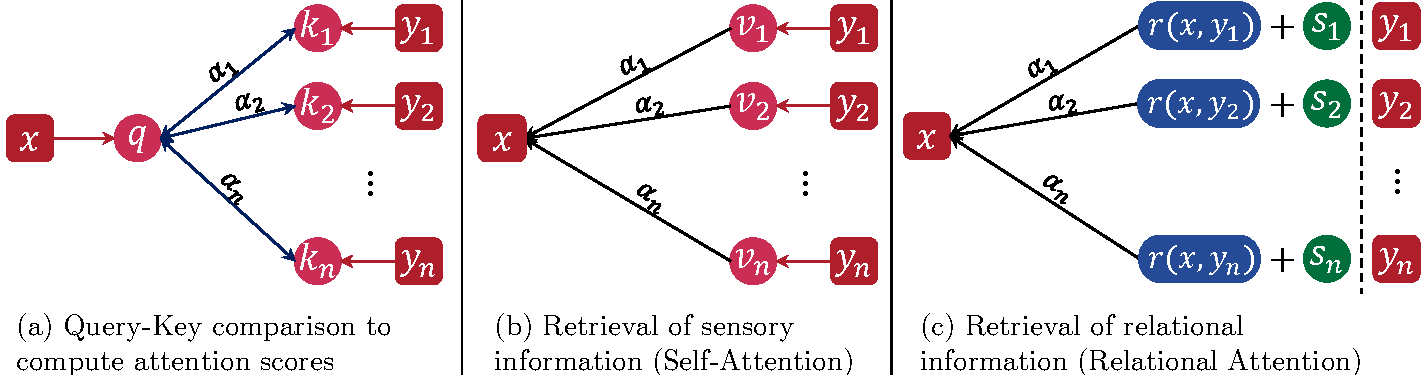
\includegraphics[width=\textwidth]{figs/attn_fig_combined.pdf}
  \caption{A depiction of $\Attn(x, \ys)$ and $\RelAttn(x, \ys)$. Both forms start with a query-key comparison to select objects to attend to. Self-attention retrieves sensory information on the attributes of individual objects while relational attention retrieves relational information on the relation between the attended objects and the receiver.}\label{fig:selfattn_relattn}
\end{figure}
